\documentclass[tikz, border=10pt]{standalone}
\usepackage{amsmath}
\usepackage{amssymb}
\usetikzlibrary{shapes.geometric, arrows.meta, positioning, calc, backgrounds, fit}

\begin{document}
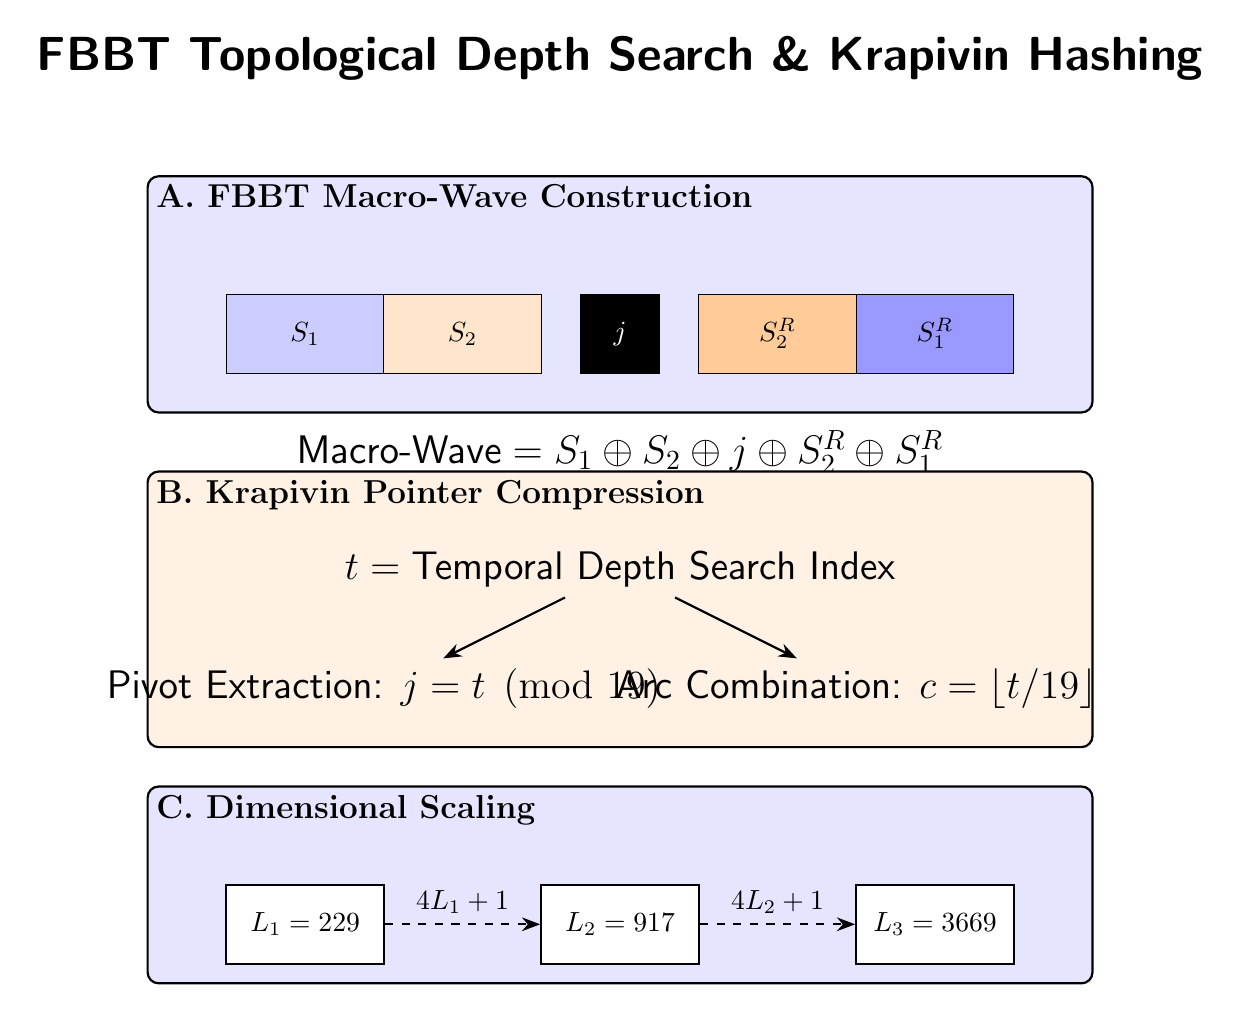
\begin{tikzpicture}[
    font=\sffamily,
    >=Stealth,
    box/.style={draw, rounded corners, fill=white, thick, minimum width=3cm, minimum height=1cm, align=center},
    highlight_box/.style={draw, rounded corners, fill=blue!10, thick, minimum width=3cm, minimum height=1cm, align=center},
    orange_box/.style={draw, rounded corners, fill=orange!10, thick, minimum width=3cm, minimum height=1cm, align=center},
    math/.style={font=\sffamily\Large}
]

% BACKGROUND GRID (Optional for visual structure, but let's just use nodes)

% TITLE
\node[font=\sffamily\LARGE\bfseries] (title) at (0, 7) {FBBT Topological Depth Search \& Krapivin Hashing};

% SECTION A: FBBT Macro-Wave
\node[highlight_box, minimum width=12cm, minimum height=3cm] (sectA) at (0, 4) {};
\node[anchor=north west, font=\bfseries] at (sectA.north west) {\large A. FBBT Macro-Wave Construction};

% Blocks inside Section A
\node[draw, fill=blue!20, minimum width=2cm, minimum height=1cm] (s1) at (-4, 3.5) {$S_1$};
\node[draw, fill=orange!20, minimum width=2cm, minimum height=1cm] (s2) at (-2, 3.5) {$S_2$};
\node[draw, fill=black, text=white, minimum width=1cm, minimum height=1cm] (pivot) at (0, 3.5) {$j$};
\node[draw, fill=orange!40, minimum width=2cm, minimum height=1cm] (s2r) at (2, 3.5) {$S_2^R$};
\node[draw, fill=blue!40, minimum width=2cm, minimum height=1cm] (s1r) at (4, 3.5) {$S_1^R$};

\node[math] at (0, 2) {$\text{Macro-Wave} = S_1 \oplus S_2 \oplus j \oplus S_2^R \oplus S_1^R$};

% SECTION B: Krapivin Compression
\node[orange_box, minimum width=12cm, minimum height=3.5cm] (sectB) at (0, 0) {};
\node[anchor=north west, font=\bfseries] at (sectB.north west) {\large B. Krapivin Pointer Compression};

\node[math] (krapivin_t) at (0, 0.5) {$t = \text{Temporal Depth Search Index}$};
\node[math] (krapivin_j) at (-3, -1) {Pivot Extraction: $j = t \pmod{19}$};
\node[math] (krapivin_c) at (3, -1) {Arc Combination: $c = \lfloor t / 19 \rfloor$};

\draw[->, thick] (krapivin_t) -- (krapivin_j);
\draw[->, thick] (krapivin_t) -- (krapivin_c);

% SECTION C: Dimensional Scaling
\node[highlight_box, minimum width=12cm, minimum height=2.5cm] (sectC) at (0, -3.5) {};
\node[anchor=north west, font=\bfseries] at (sectC.north west) {\large C. Dimensional Scaling};

\node[draw, fill=white, thick, minimum width=2cm, minimum height=1cm] (L229) at (-4, -4) {$L_1 = 229$};
\node[draw, fill=white, thick, minimum width=2cm, minimum height=1cm] (L917) at (0, -4) {$L_2 = 917$};
\node[draw, fill=white, thick, minimum width=2cm, minimum height=1cm] (L3669) at (4, -4) {$L_3 = 3669$};

\draw[->, thick, dashed] (L229) -- node[above] {$4 L_1 + 1$} (L917);
\draw[->, thick, dashed] (L917) -- node[above] {$4 L_2 + 1$} (L3669);

\end{tikzpicture}
\end{document}
